\documentclass[11pt,]{article}
\usepackage[]{mathpazo}
\usepackage{amssymb,amsmath}
\usepackage{ifxetex,ifluatex}
\usepackage{fixltx2e} % provides \textsubscript
\ifnum 0\ifxetex 1\fi\ifluatex 1\fi=0 % if pdftex
  \usepackage[T1]{fontenc}
  \usepackage[utf8]{inputenc}
\else % if luatex or xelatex
  \ifxetex
    \usepackage{mathspec}
  \else
    \usepackage{fontspec}
  \fi
  \defaultfontfeatures{Ligatures=TeX,Scale=MatchLowercase}
\fi
% use upquote if available, for straight quotes in verbatim environments
\IfFileExists{upquote.sty}{\usepackage{upquote}}{}
% use microtype if available
\IfFileExists{microtype.sty}{%
\usepackage{microtype}
\UseMicrotypeSet[protrusion]{basicmath} % disable protrusion for tt fonts
}{}
\usepackage[margin=1in]{geometry}
\usepackage{hyperref}
\hypersetup{unicode=true,
            pdftitle={Case Study: Predicting the outcomes of the 2017 Dutch General Elections},
            pdfauthor={Ilse van Beelen, Floor Komen},
            pdfkeywords={put some keywords here},
            pdfborder={0 0 0},
            breaklinks=true}
\urlstyle{same}  % don't use monospace font for urls
\usepackage{natbib}
\bibliographystyle{plainnat}
\usepackage{color}
\usepackage{fancyvrb}
\newcommand{\VerbBar}{|}
\newcommand{\VERB}{\Verb[commandchars=\\\{\}]}
\DefineVerbatimEnvironment{Highlighting}{Verbatim}{commandchars=\\\{\}}
% Add ',fontsize=\small' for more characters per line
\usepackage{framed}
\definecolor{shadecolor}{RGB}{248,248,248}
\newenvironment{Shaded}{\begin{snugshade}}{\end{snugshade}}
\newcommand{\KeywordTok}[1]{\textcolor[rgb]{0.13,0.29,0.53}{\textbf{#1}}}
\newcommand{\DataTypeTok}[1]{\textcolor[rgb]{0.13,0.29,0.53}{#1}}
\newcommand{\DecValTok}[1]{\textcolor[rgb]{0.00,0.00,0.81}{#1}}
\newcommand{\BaseNTok}[1]{\textcolor[rgb]{0.00,0.00,0.81}{#1}}
\newcommand{\FloatTok}[1]{\textcolor[rgb]{0.00,0.00,0.81}{#1}}
\newcommand{\ConstantTok}[1]{\textcolor[rgb]{0.00,0.00,0.00}{#1}}
\newcommand{\CharTok}[1]{\textcolor[rgb]{0.31,0.60,0.02}{#1}}
\newcommand{\SpecialCharTok}[1]{\textcolor[rgb]{0.00,0.00,0.00}{#1}}
\newcommand{\StringTok}[1]{\textcolor[rgb]{0.31,0.60,0.02}{#1}}
\newcommand{\VerbatimStringTok}[1]{\textcolor[rgb]{0.31,0.60,0.02}{#1}}
\newcommand{\SpecialStringTok}[1]{\textcolor[rgb]{0.31,0.60,0.02}{#1}}
\newcommand{\ImportTok}[1]{#1}
\newcommand{\CommentTok}[1]{\textcolor[rgb]{0.56,0.35,0.01}{\textit{#1}}}
\newcommand{\DocumentationTok}[1]{\textcolor[rgb]{0.56,0.35,0.01}{\textbf{\textit{#1}}}}
\newcommand{\AnnotationTok}[1]{\textcolor[rgb]{0.56,0.35,0.01}{\textbf{\textit{#1}}}}
\newcommand{\CommentVarTok}[1]{\textcolor[rgb]{0.56,0.35,0.01}{\textbf{\textit{#1}}}}
\newcommand{\OtherTok}[1]{\textcolor[rgb]{0.56,0.35,0.01}{#1}}
\newcommand{\FunctionTok}[1]{\textcolor[rgb]{0.00,0.00,0.00}{#1}}
\newcommand{\VariableTok}[1]{\textcolor[rgb]{0.00,0.00,0.00}{#1}}
\newcommand{\ControlFlowTok}[1]{\textcolor[rgb]{0.13,0.29,0.53}{\textbf{#1}}}
\newcommand{\OperatorTok}[1]{\textcolor[rgb]{0.81,0.36,0.00}{\textbf{#1}}}
\newcommand{\BuiltInTok}[1]{#1}
\newcommand{\ExtensionTok}[1]{#1}
\newcommand{\PreprocessorTok}[1]{\textcolor[rgb]{0.56,0.35,0.01}{\textit{#1}}}
\newcommand{\AttributeTok}[1]{\textcolor[rgb]{0.77,0.63,0.00}{#1}}
\newcommand{\RegionMarkerTok}[1]{#1}
\newcommand{\InformationTok}[1]{\textcolor[rgb]{0.56,0.35,0.01}{\textbf{\textit{#1}}}}
\newcommand{\WarningTok}[1]{\textcolor[rgb]{0.56,0.35,0.01}{\textbf{\textit{#1}}}}
\newcommand{\AlertTok}[1]{\textcolor[rgb]{0.94,0.16,0.16}{#1}}
\newcommand{\ErrorTok}[1]{\textcolor[rgb]{0.64,0.00,0.00}{\textbf{#1}}}
\newcommand{\NormalTok}[1]{#1}
\usepackage{graphicx,grffile}
\makeatletter
\def\maxwidth{\ifdim\Gin@nat@width>\linewidth\linewidth\else\Gin@nat@width\fi}
\def\maxheight{\ifdim\Gin@nat@height>\textheight\textheight\else\Gin@nat@height\fi}
\makeatother
% Scale images if necessary, so that they will not overflow the page
% margins by default, and it is still possible to overwrite the defaults
% using explicit options in \includegraphics[width, height, ...]{}
\setkeys{Gin}{width=\maxwidth,height=\maxheight,keepaspectratio}
\IfFileExists{parskip.sty}{%
\usepackage{parskip}
}{% else
\setlength{\parindent}{0pt}
\setlength{\parskip}{6pt plus 2pt minus 1pt}
}
\setlength{\emergencystretch}{3em}  % prevent overfull lines
\providecommand{\tightlist}{%
  \setlength{\itemsep}{0pt}\setlength{\parskip}{0pt}}
\setcounter{secnumdepth}{0}
% Redefines (sub)paragraphs to behave more like sections
\ifx\paragraph\undefined\else
\let\oldparagraph\paragraph
\renewcommand{\paragraph}[1]{\oldparagraph{#1}\mbox{}}
\fi
\ifx\subparagraph\undefined\else
\let\oldsubparagraph\subparagraph
\renewcommand{\subparagraph}[1]{\oldsubparagraph{#1}\mbox{}}
\fi

%%% Use protect on footnotes to avoid problems with footnotes in titles
\let\rmarkdownfootnote\footnote%
\def\footnote{\protect\rmarkdownfootnote}

%%% Change title format to be more compact
\usepackage{titling}

% Create subtitle command for use in maketitle
\newcommand{\subtitle}[1]{
  \posttitle{
    \begin{center}\large#1\end{center}
    }
}

\setlength{\droptitle}{-2em}

  \title{Case Study: Predicting the outcomes of the 2017 Dutch General Elections}
    \pretitle{\vspace{\droptitle}\centering\huge}
  \posttitle{\par}
    \author{Ilse van Beelen, Floor Komen}
    \preauthor{\centering\large\emph}
  \postauthor{\par}
      \predate{\centering\large\emph}
  \postdate{\par}
    \date{January 21, 2019}

\usepackage{float}

\begin{document}
\maketitle
\begin{abstract}
For this report demographics of Dutch municipalities are compared with
the results of the general Dutch election of 2017. The demographic
variables are the \emph{Urban index}, the \emph{fraction of highly
educated residents}, \emph{Mean income}, \emph{fraction of 60 plus
residents} in a municipality and the factor \emph{Non western}. This
factor devides municipalities in the once with less than 5\%, 5-10\% and
more than 10\% Non-western residents.The research focust on the results
for the party CDA. The goal is to find voting trends per demographic
group and to make future predictions for CDA. This goal is approached
with two different models. The first is a linear model with a log
transformation of the respons. The cross validation resulted in a Mean
Prediction Squared Error (MPSE) of 0.058. The second, is a
quasi-binomial model with the logit as link function. The found MPSE is
0.0017. It is difficult to say which model fits the data better, because
they have different significant variables. However, the logistic model
fits the underlying pattern of the data better and has a smaller MPSE.
Nonetheless, both models have their limitations and the data displayed a
large overdispersion. It is not likely that predictions for future
elections can be made with these models.
\end{abstract}

\section{1. Introduction}\label{introduction}

\subsection{1.1 Motivation}\label{motivation}

For this research, the outcome from the Dutch elections of 2017 and
demographical data are combined. All data is collected per municipality
and are well maintained and reliable. This will hopefully result in
observing voting trends per demographic group. The final goal is to
validate the model for making future prediction.

\begin{figure}
\centering
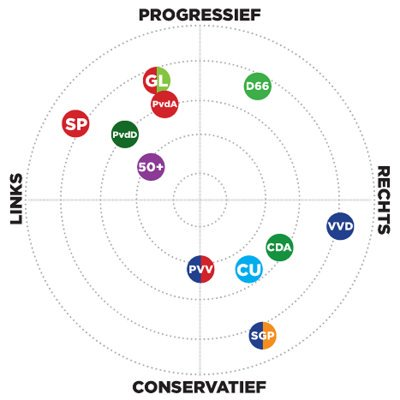
\includegraphics[width=2.60417in]{Partijlandschap.jpg}
\caption{Party landscape}
\end{figure}

\textbf{Dutch political parties}

The figure above displays the diffences between the political parties in
the Netherlands. The Netherlands has a total of 13 parties. This
research focusses on only one party. The chosen party should not be to
extreme left/right/conservative/progressive and should also be one of
the bigger parties. Otherwise, there is not enough data available,
making the results less reliable. Therefore, the party
Christen-Democratisch Appèl (CDA) is chosen.

In this research the demographics are chosen because of their influence
on a municipality level. The expectation is that a municipality with
more non-western residents for example votes different than a
municipality with less non-western residents. This is the same for the
other three demographics. Other demographics are also researched, for
example gender, but on a municipality level there is no large difference
between the amount of men and women per municipality. Gender is a more
interesting demographic to research on an individual level. \emph{The
standardized income per municipality} are given in thousands.
\emph{Urban index} of a municipality is a database with five categories
(0 to 4) per municipality. These five categories are:

\begin{itemize}
\item No urbanity (less than 500 addresses per $km^2$), score 0
\item Little urbanity (500-1000 addresses per $km^2$), score 1
\item Moderate urbanity (1000- 1500 addresses per $km^2$), score 2
\item Strong urbanity (1500-2500 addresses per $km^2$), score 3
\item Really strong urbanity (more than 2500 addresses per $km^2$), score 4
\end{itemize}

Per municipality the amount of \(km^2\) per category is given. In the
raw dataset the \emph{Non-western residents} is given as an absolute
amount per municipality. This is transformed to a fraction and later
during the data cleaning divided in three groups.

\subsection{1.2 Data sources}\label{data-sources}

\textbf{Electoral data}

For the electoral data, the results of the 2017 general election are
used. This is the most recent national election and is of the most
important election type in the Netherlands. Furthermore, it had a turnup
of 81.9\%\footnote{\url{https://www.kiesraad.nl/actueel/nieuws/2017/03/20/officiele-uitslag-tweede-kamerverkiezing-15-maart-2017}}.
Therefore, it seems plausible that the data for this election is
representative of the political makeup of different municipalities. The
raw data is directly downloaded from the official government
website\footnote{\url{https://data.overheid.nl/data/dataset/verkiezingsuitslag-tweede-kamer-2017}}
This raw dataset is a .csv file with the absolute number of votes for
every party in every municipality.

\textbf{Demographical data}

The demographical data is obtained from the CBS, the official Dutch
statistical agency.\footnote{\url{https://opendata.cbs.nl/statline/\#/CBS/nl/dataset/70072ned/table?ts=1544803364892}}.
From the wealth of demographical information available a handful of
attributes are picked that are suspected (based on prior research and
some gut feeling) to be useful as predictor variables. Five
demographical attributes were landed: education grade, average income,
age, urbanization and the amount of people with a non-western
background. The data downloaded from the CBS site usually had to be
transformed to get it in a useful predictor variable format. The
specifics of these are described in the next section.

\subsection{1.3 Data cleaning}\label{data-cleaning}

An extensive amount of data cleaning had to be done. Below these steps
are describes.

\textbf{Electoral data}

The absolute amount of votes for CDA and the total amount of votes per
municipalities are kept in the dataset, \texttt{CDA\_abs} and
\texttt{Total\_abs}, respectively. Information is removed from the other
12 parties. The variable \texttt{CDA\_frac} is created, this the
fraction of votes for CDA per munipicality.

\textbf{Demographical data}

The demographics are downloaded from CBS in multiple csv files. All
files are in a long format and are transformed to a wide format using R.
The variables \emph{highly educated}, \emph{Non western residens} and
\emph{60 plus residents} are in absolute amounts. All are transformed to
fractions. These are called, \texttt{High\_educated\_frac},
\texttt{Non\_west\_frac} and \texttt{Frac\_60plus}, respectively.

\texttt{Non\_west\_frac} does not have a large spread (for most
municipalities between 0 to 10\%). It is decided to ceate a new variable
\texttt{Non\_west} that divides the variable in three groups:

\begin{itemize}
\item Municipalities with less than 5 \% non-western residents 
\item Municipalities with 5-10 \% non-western resident 
\item Municipalities with mre than 10 \% non-western residents
\end{itemize}

Furthermore, the variables \texttt{Urban\_index} and
\texttt{Mean\_income} did not need to be transformed. All municipalities
are in \texttt{Muni}. At last, the electoral data and demographic data
are combined again. Only the municipality Boxmeer is removed, due to a
mistake not all the votes are reported here\footnote{\url{https://www.gelderlander.nl/boxmeer/7-600-stemmen-in-boxmeer-niet-meegenomen-in-uitslag-verkiezingen~a063ee9e/}}.

\begin{verbatim}
##      Muni              CDA_frac       Urban_index     High_educated_frac
##  Length:366         Min.   :0.0310   Min.   :0.0000   Min.   :0.1200    
##  Class :character   1st Qu.:0.1170   1st Qu.:0.6623   1st Qu.:0.2200    
##  Mode  :character   Median :0.1420   Median :1.2305   Median :0.2600    
##                     Mean   :0.1528   Mean   :1.4280   Mean   :0.2662    
##                     3rd Qu.:0.1820   3rd Qu.:2.1750   3rd Qu.:0.3000    
##                     Max.   :0.4200   Max.   :3.7890   Max.   :0.4700    
##   Mean_income    Non_west_frac        CDA_abs        Total_abs     
##  Min.   :20.80   Min.   :0.01000   Min.   :  421   Min.   :  2727  
##  1st Qu.:24.30   1st Qu.:0.03000   1st Qu.: 1737   1st Qu.: 11516  
##  Median :25.60   Median :0.05000   Median : 2510   Median : 16915  
##  Mean   :25.91   Mean   :0.06574   Mean   : 3254   Mean   : 25162  
##  3rd Qu.:27.00   3rd Qu.:0.08000   3rd Qu.: 4023   3rd Qu.: 27087  
##  Max.   :41.80   Max.   :0.38000   Max.   :18813   Max.   :440854  
##  Non_west  Frac_60plus    
##  1:178    Min.   :0.0700  
##  2:111    1st Qu.:0.1200  
##  3: 77    Median :0.1300  
##           Mean   :0.1327  
##           3rd Qu.:0.1400  
##           Max.   :0.1800
\end{verbatim}

The summary shows that \texttt{CDA\_frac} ranges from 0.03 to 0.42. The
three groups in \texttt{Non\_west} are not of equal size. Also
\texttt{Mean\_income} has a large range, from 20.80 to 41.80 times 1000
euros. The final dataset has no NAs.

\subsection{1.3 Data visualisation}\label{data-visualisation}

In this part the cleaned data is visualized, so that a good picture can
be obtained of the current data. First of all some demographics of data
will be showed. In figure \ref{1} of the \emph{parties}, \emph{the urban
index}, \emph{the percentage of highly educated residents}, \emph{the
mean income}, \emph{The non west residents factor} and \emph{the
percentage 60 plus} are plotted.

As visualized in figure \ref{1}, most variables are normally
distributed. Because of the low values at the x-axis, the CDA, 60 plus
percentage and the highly educated densities are above 1. The area
beneath the curve sums up to 1, so they are correct. However, the
variable \texttt{Non\_west\_frac} shows a large peak around 5\%.

\begin{figure}[H]

{\centering 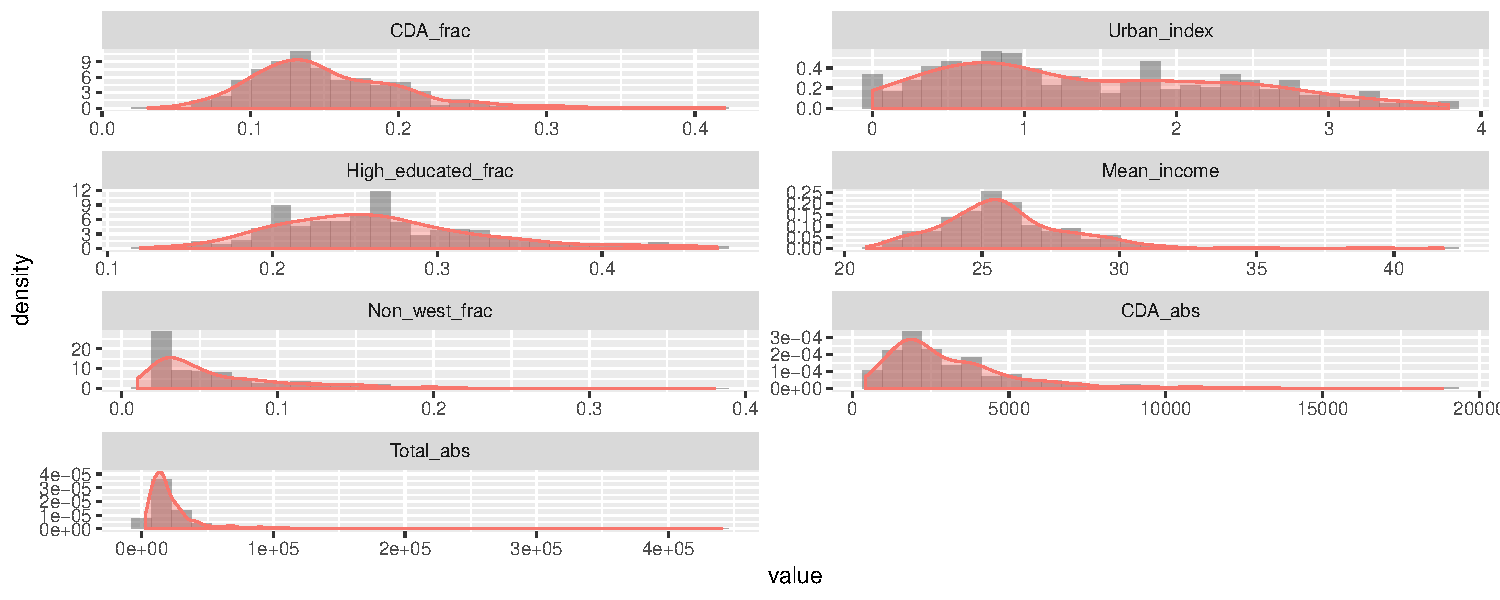
\includegraphics{Report_files/figure-latex/demographics_data-1} 

}

\caption{\label{1} Density plot}\label{fig:demographics_data}
\end{figure}

\textbf{Correlation heatmap}

In this heatmap (figure \ref{2}) the correlation between explanatory and
respons variable are showed. The red color means a positive relation,
the purple color means a negative relation. The \emph{non\_west}
variable is not taken into account, because it is a factor and the other
variables are continous. \texttt{Mean\_income} and
\texttt{High\_educated\_frac} have the strongest positive correlation
and \texttt{Urban\_index} and \texttt{CDA\_frac} have the strongest
negative correlation. None of the correlations are above 0.8, which is a
good sign.

\begin{figure}[H]

{\centering 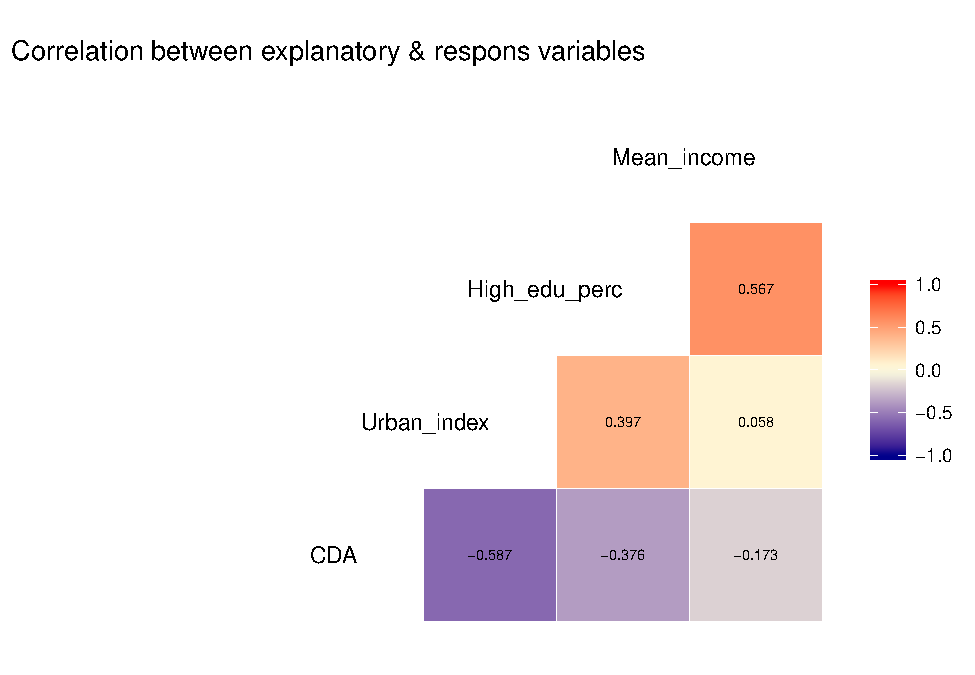
\includegraphics{Report_files/figure-latex/correlation_heatmap-1} 

}

\caption{\label{2}Correlation between explanatory and respons variables}\label{fig:correlation_heatmap}
\end{figure}

\textbf{Scatter plots of correlations }

The strongest correlations in figure \ref{2} are again visualized in
scatterplots. The visible trend is that when the the urbanity index goes
up, the votes for CDA goes down. A similar trend is visible for 60 plus
residents. The observations of the 60 plus residents seem to follow a
horizontal line pattern. This is due to rounding.

\begin{figure}[H]

{\centering 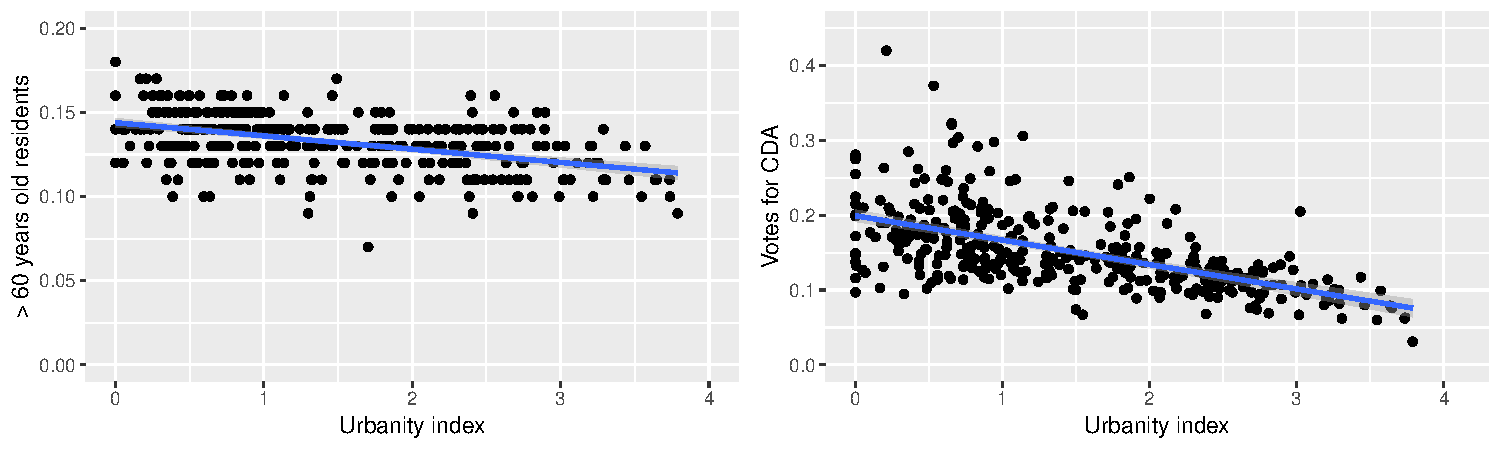
\includegraphics{Report_files/figure-latex/unnamed-chunk-5-1} 

}

\caption{\label{3}Scatterplots strongest correlations}\label{fig:unnamed-chunk-5}
\end{figure}

Figure \ref{5} visualized that when the mean income goes up, the
fraction highly educated also goes up. Most municipalities are scattered
around an income of 20 to 30 thousand euros, but three municipalities
stand out with a mean income around 40 thousand. Also, when the urbanity
index increases the fraction highly educated residents increases, but
here none of the municipalities stand out.

\begin{figure}[H]

{\centering 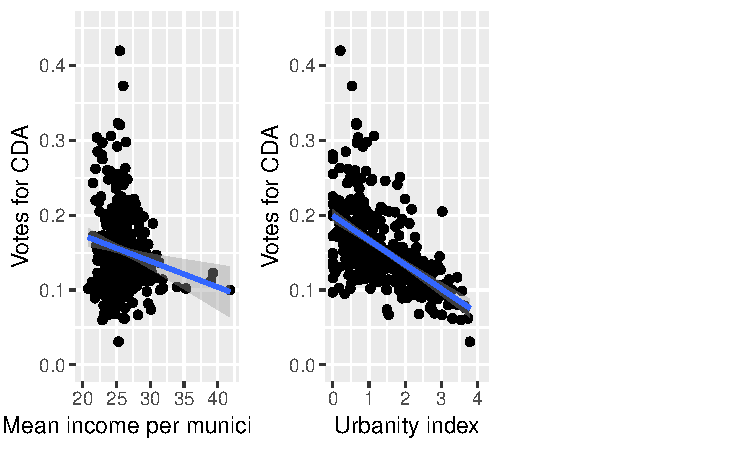
\includegraphics{Report_files/figure-latex/unnamed-chunk-6-1} 

}

\caption{\label{5}Scatterplot strongest correlations}\label{fig:unnamed-chunk-6}
\end{figure}

\textbf{Multiple boxplots}

In this graph boxplots are made, to compare the variable
\texttt{Non\_west} with \texttt{Urbanity\_index} and \texttt{CDA\_frac}.
A boxplot is a standardized way to display the distribution of data. It
gives the minimum, first quartile, median, third quartile and the
maximum. If there are any outliers, the boxplot is extended with those.
The line within the box is the median, the first and third quartile are
the down- and upside of the box, respectively. The length of the box is
the Inter Quartile Range (IQR). The minimum and maximum are 1.5X Inter
Quartile Range (IQR). Observations further away can be considered
outliers.

\begin{figure}[H]

{\centering 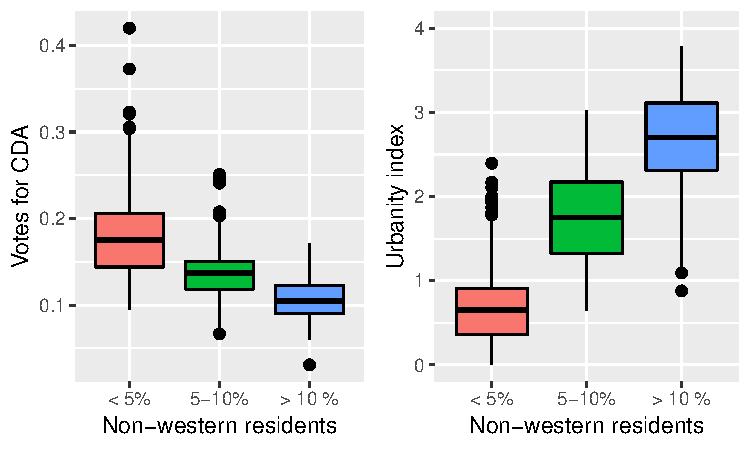
\includegraphics{Report_files/figure-latex/unnamed-chunk-7-1} 

}

\caption{\label{6}Three boxplots: Boxplot of Non-west against votes for CDA and Urbanity index}\label{fig:unnamed-chunk-7}
\end{figure}

Figure \ref{6} visualizes that the Non-western residents tend to live in
municipalities with a high Urban Index and vote less for CDA. A few
possible outliers are seen in the boxplot for municipalities with less
than 5\% Non-western residents.

\section{2. Multiple linear
regression}\label{multiple-linear-regression}

In this chapter multiple linear models are generated. The demographics
tested in this model are the highly educated fraction in a municipality
\texttt{High\_educated\_frac}, the urban index of a municipality
\texttt{Urban\_index}, the mean income of the municipality
\texttt{Mean\_income}, the non-west factor \texttt{Non\_west} and the
fraction that is 60 plus in the municipality \texttt{Frac\_60plus}. The
error assumptions are also discussed. This are assumptions made for the
residuals, to check if meet the requirements for correct linear
regressions. These assumptions are:

\begin{itemize}
\item Linearity: The expected value of the error is zero, $E(\epsilon) = 0$
\item Constant variance: The variance of the error is constant 
\item Normality: The errors are normally distributed
\item Indepence: The observations are sampled independently
\end{itemize}

\subsection{2.1 First model}\label{first-model}

The first model will be the model with all the demographics:\\
\(Y_i = \beta_0 + \beta_1*high Educated Fraction + \beta_2*Urban Index + \beta_3*Mean Income + \beta_4*Non West2 +\beta_5*Non West3 + \beta_6*Frac 60plus + \epsilon_i\)

With \(i = 1, 2,.., N\) for the number of observations. The outcome of
this model is shown below:

\begin{table}[ht]
\centering
\begin{tabular}{rrrrr}
  \hline
 & Estimate & Std. Error & t value & Pr() \\ 
  \hline
(Intercept) & 0.3381 & 0.0314 & 10.78 & 0.0000 \\ 
  High\_educated\_frac & -0.0864 & 0.0454 & -1.90 & 0.0576 \\ 
  Urban\_index & -0.0193 & 0.0041 & -4.69 & 0.0000 \\ 
  Mean\_income & -0.0015 & 0.0011 & -1.46 & 0.1453 \\ 
  Non\_west2 & -0.0223 & 0.0065 & -3.45 & 0.0006 \\ 
  Non\_west3 & -0.0455 & 0.0095 & -4.77 & 0.0000 \\ 
  Frac\_60plus & -0.5904 & 0.1494 & -3.95 & 0.0001 \\ 
   \hline
\end{tabular}
\end{table}

The first model is the full model, \texttt{High\_educated\_frac} and
\texttt{Mean\_income} do not have a significant t-value. Before any
conclusions are made, the assumptions are checked via plots and the VIF
is checked. The VIF is the Variation Inflation Factor, it implies if
there is multicollinearity between variables. The formula for VIF is
\(1/(1-R^2)\) and the thresholdvalue is 10. Meaning that values above 10
give signs of multicollinearity. As shown below none of the values are
above 10, so no signs of collinearity.

\begin{verbatim}
## High_educated_frac        Urban_index        Mean_income 
##           1.871032           3.383149           1.658015 
##          Non_west2          Non_west3        Frac_60plus 
##           1.974537           3.361734           1.289979
\end{verbatim}

\begin{verbatim}
## [1]  74 298
\end{verbatim}

\begin{figure}[H]

{\centering 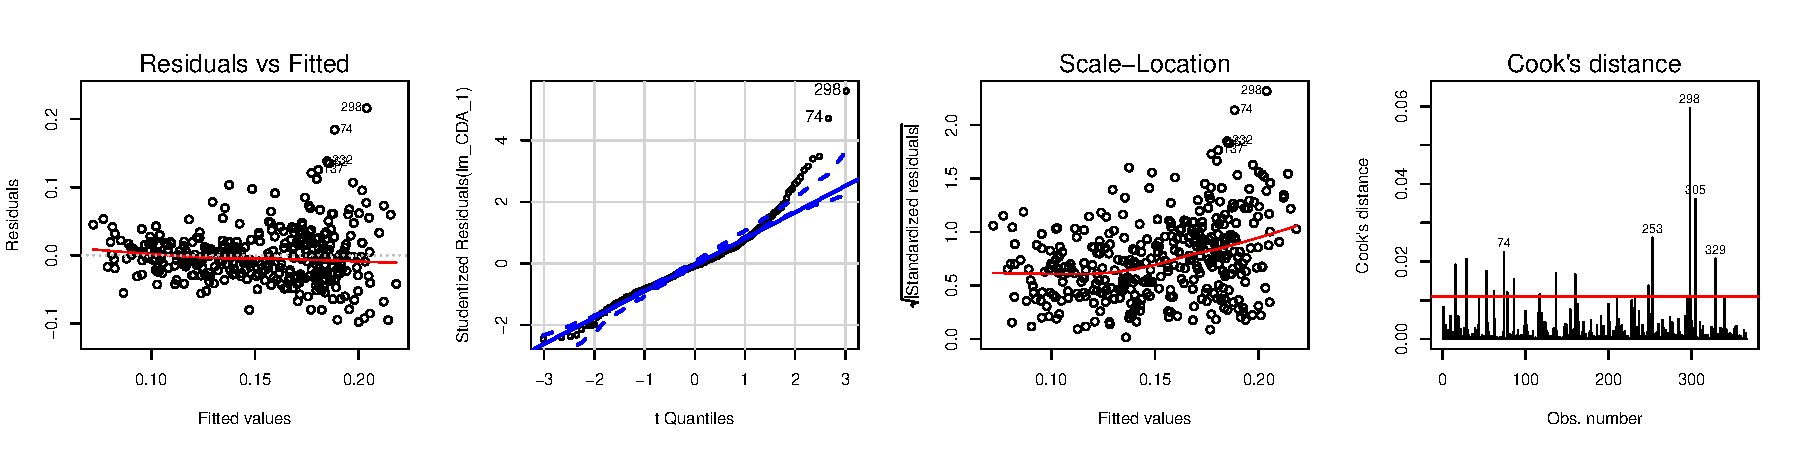
\includegraphics{Report_files/figure-latex/unnamed-chunk-8-1} 

}

\caption{\label{afm}assumptions first model}\label{fig:unnamed-chunk-8}
\end{figure}

In figure \ref{afm} four diagnostics plots are shown. The first plot
(Residuals vs Fitted) shows that the residuals have a `loudspeaker
pattern', the variance of the residuals tends to increase with an
increase of the fitted value. Because of this, a BoxCox graph is
consulted. This graph suggests a transformation for the response. The
BoxCox in figure \ref{BC1} has a 95\% Confidence interval located around
the 0. Hence, a log transformation is suggested.

\begin{figure}[H]

{\centering 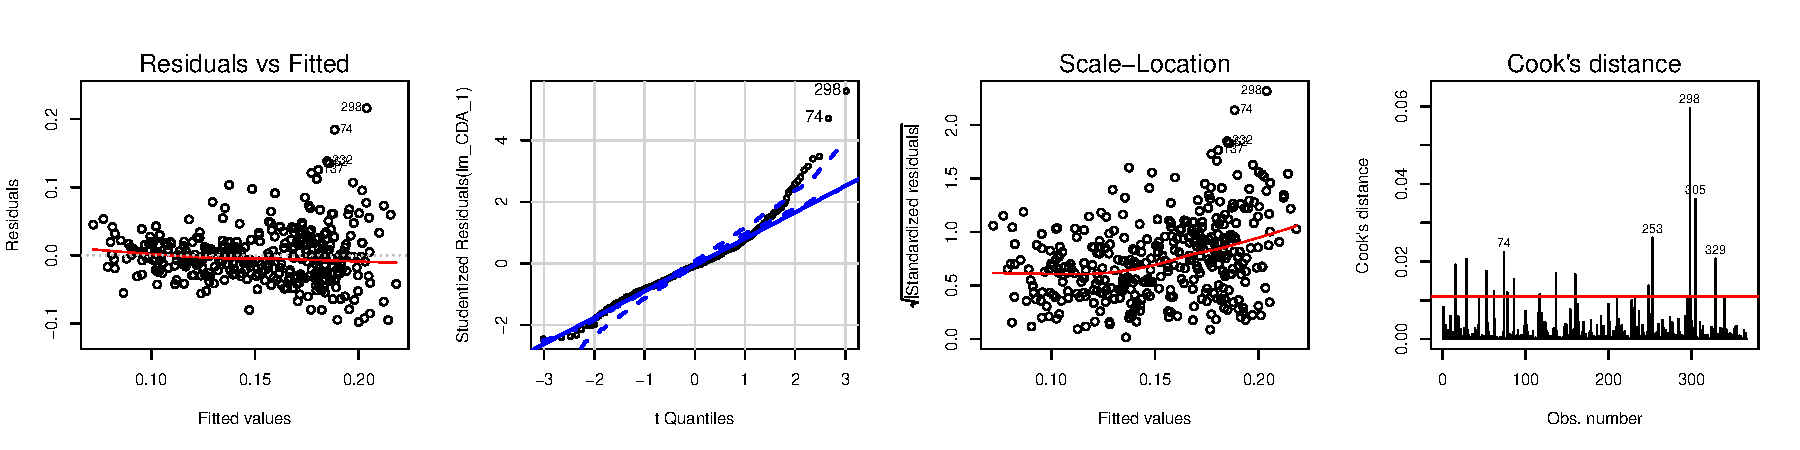
\includegraphics{Report_files/figure-latex/unnamed-chunk-9-1} 

}

\caption{\label{BC1}BoxCox first model}\label{fig:unnamed-chunk-9}
\end{figure}

\subsection{2.2 Second model}\label{second-model}

In the second model the response variable will be ln transformed. So the
new model will be:\\
\(ln(Y_i) = \beta_0 + \beta_1 \cdot high educated fraction + \beta_2 \cdot Urban index + \beta_3 \cdot Mean income + \beta_4 \cdot Non west2 + \beta_5 \cdot Non west 3 + \beta_6 \cdot Frac 60plus + \epsilon_i\)

\begin{table}[ht]
\centering
\begin{tabular}{rrrrr}
  \hline
 & Estimate & Std. Error & t value & Pr() \\ 
  \hline
(Intercept) & -0.9944 & 0.1882 & -5.28 & 0.0000 \\ 
  High\_educated\_frac & -0.8808 & 0.2723 & -3.24 & 0.0013 \\ 
  Urban\_index & -0.1388 & 0.0247 & -5.62 & 0.0000 \\ 
  Mean\_income & -0.0024 & 0.0064 & -0.38 & 0.7042 \\ 
  Non\_west2 & -0.0991 & 0.0389 & -2.55 & 0.0112 \\ 
  Non\_west3 & -0.2763 & 0.0572 & -4.83 & 0.0000 \\ 
  Frac\_60plus & -2.6940 & 0.8965 & -3.01 & 0.0028 \\ 
   \hline
\end{tabular}
\end{table}

\begin{verbatim}
## [1]  16 237
\end{verbatim}

\begin{figure}[H]

{\centering 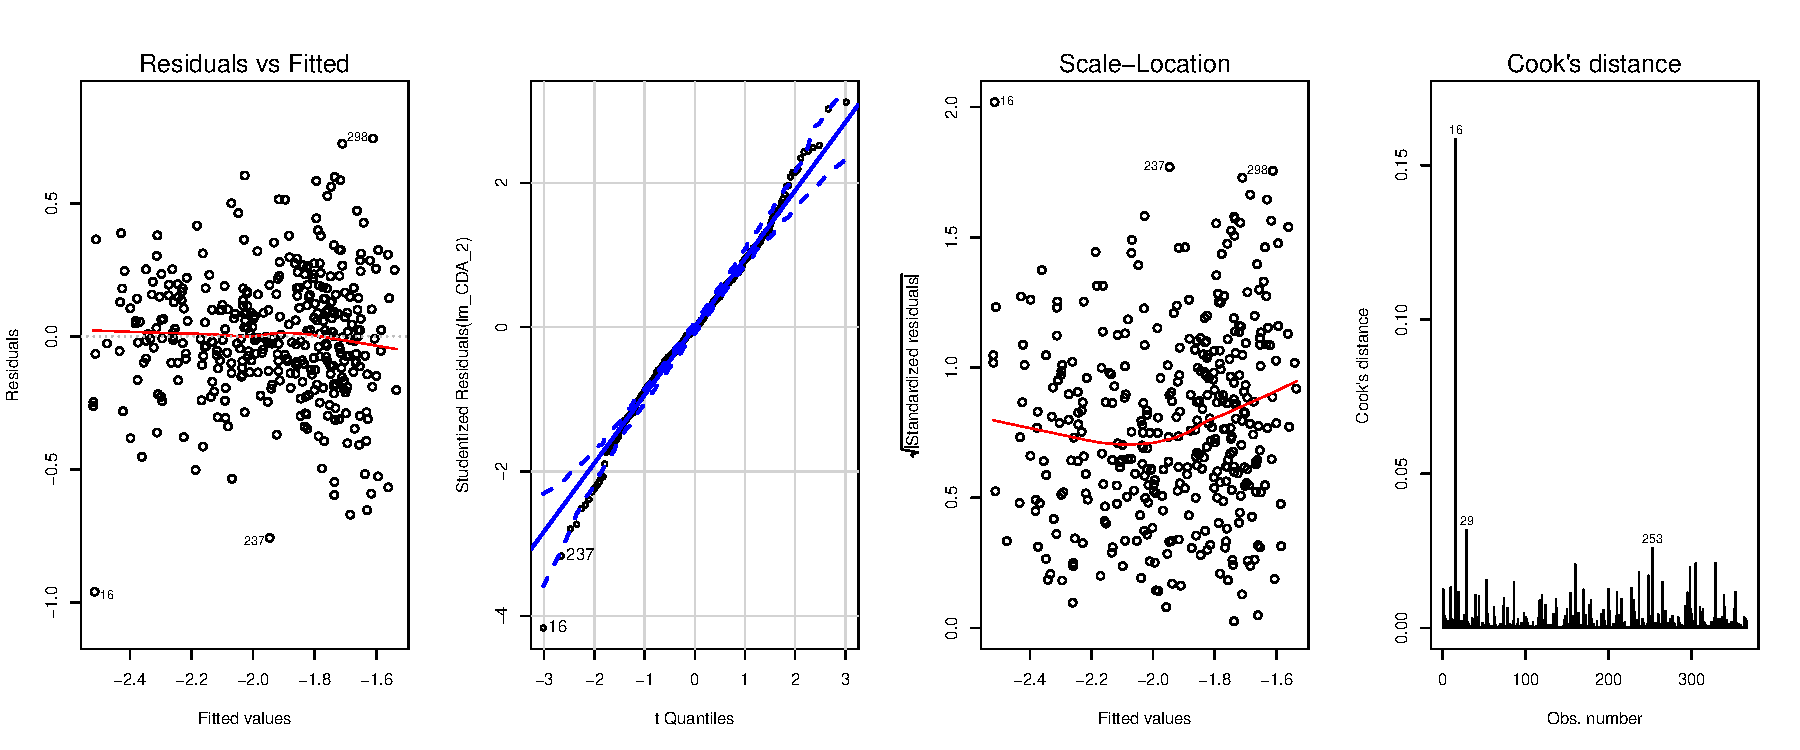
\includegraphics{Report_files/figure-latex/unnamed-chunk-10-1} 

}

\caption{\label{asm}Diagnostics plot second model}\label{fig:unnamed-chunk-10}
\end{figure}

The plots in figure \ref{asm} show one large outlier, the municipality
Amsterdam (obs 16). Amsterdams value for the cooks distance goes far
above the cutoff value, \(4/(369-5-1)=0.011\). It is also outside the
(-3,3) range with the studentized residuals. This is strong evidence
that this municipality is an outlier and should be removed.

For the second model without Amsterdam, a step function is used. This
step function uses the Aikaike Information Criterion (AIC) for backward
elimination and shows which variable should be removed to decrease the
AIC. The formula for AIC is \(AIC=-2log(likelihood)+2p\), p is the
number of parameters in the model. The variables that are left are the
variables used in the final model.

\begin{verbatim}
## Start:  AIC=-1041.5
## log(CDA_frac) ~ High_educated_frac + Urban_index + Mean_income + 
##     Non_west + Frac_60plus
## 
##                      Df Sum of Sq    RSS     AIC
## - Mean_income         1   0.04208 20.291 -1042.7
## <none>                            20.249 -1041.5
## - High_educated_frac  1   0.36195 20.611 -1037.0
## - Frac_60plus         1   0.67266 20.922 -1031.6
## - Non_west            2   1.54236 21.792 -1018.7
## - Urban_index         1   1.72696 21.976 -1013.6
## 
## Step:  AIC=-1042.74
## log(CDA_frac) ~ High_educated_frac + Urban_index + Non_west + 
##     Frac_60plus
## 
##                      Df Sum of Sq    RSS     AIC
## <none>                            20.291 -1042.7
## - Frac_60plus         1   0.66435 20.956 -1033.0
## - High_educated_frac  1   0.85427 21.146 -1029.7
## - Non_west            2   1.51164 21.803 -1020.5
## - Urban_index         1   1.68687 21.978 -1015.6
\end{verbatim}

\begin{verbatim}
## 
## Call:
## lm(formula = log(CDA_frac) ~ High_educated_frac + Urban_index + 
##     Non_west + Frac_60plus, data = Data_CDA[-16, ])
## 
## Coefficients:
##        (Intercept)  High_educated_frac         Urban_index  
##            -1.0298             -0.8277             -0.1311  
##          Non_west2           Non_west3         Frac_60plus  
##            -0.1141             -0.2871             -3.0168
\end{verbatim}

\subsection{2.3 Final model}\label{final-model}

The backward elimination resulted in the final model.\\
\(ln(Y_i) = \beta_0 + \beta_1 \cdot high educated fraction + \beta_2 \cdot Urban index + \beta_4 \cdot Non west2 + \beta_5 \cdot Non west 3 + \beta_6 \cdot Frac 60plus + \epsilon_i\)

The coëfficients are given in the table below

\begin{table}[ht]
\centering
\begin{tabular}{rrrrr}
  \hline
 & Estimate & Std. Error & t value & Pr($>$$|$t$|$) \\ 
  \hline
(Intercept) & -1.0298 & 0.1365 & -7.54 & 0.0000 \\ 
  High\_educated\_frac & -0.8277 & 0.2129 & -3.89 & 0.0001 \\ 
  Urban\_index & -0.1311 & 0.0240 & -5.46 & 0.0000 \\ 
  Non\_west2 & -0.1141 & 0.0378 & -3.02 & 0.0027 \\ 
  Non\_west3 & -0.2871 & 0.0559 & -5.13 & 0.0000 \\ 
  Frac\_60plus & -3.0168 & 0.8799 & -3.43 & 0.0007 \\ 
   \hline
\end{tabular}
\end{table}

\begin{verbatim}
## 237 298 
## 236 297
\end{verbatim}

\begin{figure}[H]

{\centering 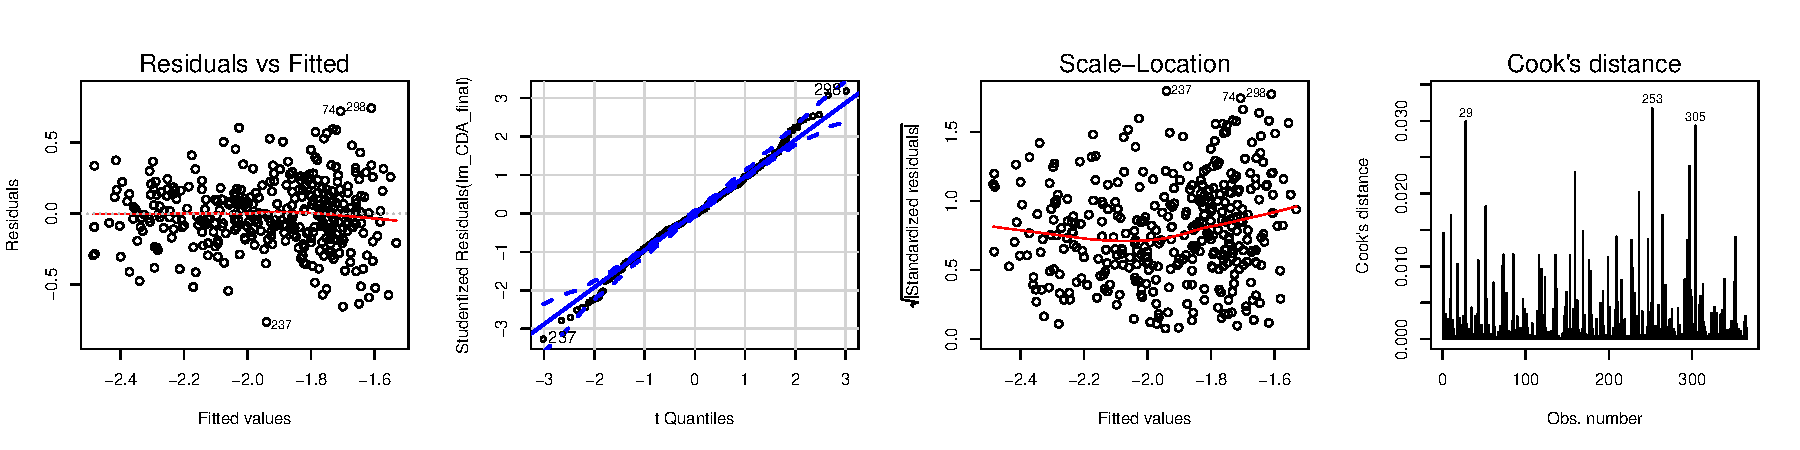
\includegraphics{Report_files/figure-latex/unnamed-chunk-12-1} 

}

\caption{\label{asm2}Assumptions second model}\label{fig:unnamed-chunk-12}
\end{figure}

The estimates for the predictors are filled in the model and the
following results are obtained:

\(ln(Y_i) = -1.0298 -0.8277 \cdot High Educated fraction -0.1311 \cdot Urban Index -0.1141 \cdot Non West2 -0.2871 \cdot Non West3 -3.0168 \cdot Frac 60plus + \epsilon_i\)

All the coëfficients are negative, but because the fitted value is a log
value the response will be positive.

\subsection{2.4 Cross validation}\label{cross-validation}

To tell something about the prediction possibilities of the model, cross
validation is done. Cross validation helps to discover how well the
model predicts on average. Cross validation estimates the Mean Squared
Prediction Error (MPSE) of a model.

The following steps are done. First 5k-folds are made, meaning that the
data is divided in five folds. Next, a loss function is created This
function finds the square of the difference between the observed value
\(Y_i\) predicted value \(\widehat{Y_i}\). Afterwards the sum is taken
and divided by the length of the folds, to correct for the length of
each fold. The formula below shows the loss function:

\(\frac{(Y_i - \widehat{Y_i})^2}{length(fold)}\)

Four of the five k-folds are used to train the data, the other one is
the test data. The model is fitted on the training data and afterwards
it tries to fit on the test data, to see if it predicts closely. This is
done 5 times, every time another fold is the test data. As is shown
below, the MSPE is 0.0582.

\begin{Shaded}
\begin{Highlighting}[]
\NormalTok{lm_CDA_final <-}\StringTok{ }\KeywordTok{lm}\NormalTok{(}\KeywordTok{log}\NormalTok{(CDA_frac) }\OperatorTok{~}\StringTok{ }\NormalTok{High_educated_frac }\OperatorTok{+}\StringTok{ }\NormalTok{Urban_index }\OperatorTok{+}\StringTok{ }\NormalTok{Non_west }\OperatorTok{+}\StringTok{ }
\StringTok{    }\NormalTok{Frac_60plus, }\DataTypeTok{data =}\NormalTok{ Data_CDA[}\OperatorTok{-}\DecValTok{16}\NormalTok{, ])}
\NormalTok{K <-}\StringTok{ }\DecValTok{5}
\NormalTok{index <-}\StringTok{ }\KeywordTok{rep}\NormalTok{(}\DecValTok{1}\OperatorTok{:}\NormalTok{K, }\KeywordTok{floor}\NormalTok{(}\KeywordTok{nrow}\NormalTok{(Data_CDA)}\OperatorTok{/}\NormalTok{K) }\OperatorTok{+}\StringTok{ }\DecValTok{1}\NormalTok{)[}\DecValTok{1}\OperatorTok{:}\KeywordTok{nrow}\NormalTok{(Data_CDA)]}
\NormalTok{fold.index <-}\StringTok{ }\KeywordTok{sample}\NormalTok{(index)}
\NormalTok{Loss <-}\StringTok{ }\ControlFlowTok{function}\NormalTok{(x, y) \{}
    \KeywordTok{sum}\NormalTok{((x }\OperatorTok{-}\StringTok{ }\NormalTok{y)}\OperatorTok{^}\DecValTok{2}\NormalTok{)}\OperatorTok{/}\KeywordTok{length}\NormalTok{(x)}
\NormalTok{\}}
\NormalTok{loss <-}\StringTok{ }\KeywordTok{numeric}\NormalTok{(K)}
\ControlFlowTok{for}\NormalTok{ (k }\ControlFlowTok{in} \DecValTok{1}\OperatorTok{:}\NormalTok{K) \{}
\NormalTok{    training <-}\StringTok{ }\NormalTok{Data_CDA[fold.index }\OperatorTok{!=}\StringTok{ }\NormalTok{k, ]}
\NormalTok{    validation <-}\StringTok{ }\NormalTok{Data_CDA[fold.index }\OperatorTok{==}\StringTok{ }\NormalTok{k, ]}
\NormalTok{    training.fit <-}\StringTok{ }\NormalTok{lm_CDA_final}
\NormalTok{    validation.predict <-}\StringTok{ }\KeywordTok{predict}\NormalTok{(training.fit, }\DataTypeTok{newdata =}\NormalTok{ validation, }\DataTypeTok{type =} \StringTok{"response"}\NormalTok{)}
\NormalTok{    loss[k] <-}\StringTok{ }\KeywordTok{Loss}\NormalTok{(}\KeywordTok{log}\NormalTok{(validation}\OperatorTok{$}\NormalTok{CDA_frac), validation.predict)}
\NormalTok{\}}
\KeywordTok{mean}\NormalTok{(loss)}
\end{Highlighting}
\end{Shaded}

\begin{verbatim}
## [1] 0.0581487
\end{verbatim}

\section{3. Logistic regression}\label{logistic-regression}

The raw respons variable is the absolute amount of residents per
municipality that voted for CDA. For linear regresssion, this variable
is transformed to a fraction. However, the absolute total amount of
votes per municipality is also available. Therefore, a binomial model
would be a better fit to the data. A second model is developed that uses
the logit as link function to transform the range of the respons. The
choice for the logit was easily made. Because the inverse of the logit
is directly interpretable as the log-odds ratio and this link displays
the underlaying pattern of the data best. Below, the formula for the
link function:

\(\eta = log(\frac{\theta}{1 - \theta}) = \beta_0 + \beta_1 \cdot x_1 + \beta_2 \cdot x_2 + ... + \beta_n \cdot x_n\)

The ratio is the log odds that \(Y_i\) = 1 (the odds of voting for CDA).

Also for logistics regression diagnostic plots are needed to visualise
the deviance/pearson residuals and search for outliers. Most of the
diagnostics from the linear model extend relatively straighforward to
logistic regression. However, leverages are no longer just a function of
the explanatory variable, but also depend on the respons due to the
iterated weighted least squares. Furthermore, \(\theta\) can never be
zero or one. Fortunately, this was not the case for any of the
observations in this dataset.

\subsection{3.1 First model}\label{first-model-1}

Again, the first model is the full model. Stepwise backward elimination
is used to find the optimal model. Below, the formula for the full
model:

\(log(\frac{\theta_i}{1 - \theta_i}) = \beta_0 + \beta_1 \cdot UrbanIndex + \beta_2 \cdot HighlyEducatedFraction + \beta_3 \cdot MeanIncome + \beta_4 \cdot NonWest + \beta_5 \cdot Fraction60Plus + \epsilon_i\)

With \(i = 1, 2,.., N\) for the number of observations.

Below the summary of this model:

\begin{table}[ht]
\centering
\begin{tabular}{rrrrr}
  \hline
 & Estimate & Std. Error & z value & Pr($>$$|$z$|$) \\ 
  \hline
(Intercept) & -1.0560 & 0.0157 & -67.29 & 0.0000 \\ 
  Urban\_index & -0.1934 & 0.0020 & -94.91 & 0.0000 \\ 
  High\_educated\_frac & -2.1028 & 0.0200 & -105.38 & 0.0000 \\ 
  Mean\_income & 0.0156 & 0.0005 & 29.32 & 0.0000 \\ 
  Non\_west2 & -0.0563 & 0.0032 & -17.81 & 0.0000 \\ 
  Non\_west3 & -0.2593 & 0.0046 & -56.26 & 0.0000 \\ 
  Frac\_60plus & -1.3424 & 0.0737 & -18.20 & 0.0000 \\ 
   \hline
\end{tabular}
\end{table}

The summary shows that the all the variables are very significant and
have small standard errors. The full model has 359 degrees of freedom
and it is expected that the residual deviance is roughly equivalent.
However, the residual deviance is far above this value. These are strong
indications that this model suffers from overdispersion. This assumption
seems reasonable, because there is a very large variance in how many
residents per municapality voted for CDA. In some municipalities only
3\% voted for CDA, while it others nearly 50\% voted for CDA. It is
concluded that a quasi-binomial would fit the data better.

\subsection{3.2 Second model}\label{second-model-1}

The second model has still all the variables, but is fitted to a
quasi-binomial. Below the output of the summary is visualized:

\begin{table}[ht]
\centering
\begin{tabular}{rrrrr}
  \hline
 & Estimate & Std. Error & t value & Pr($>$$|$t$|$) \\ 
  \hline
(Intercept) & -1.0560 & 0.2501 & -4.22 & 0.0000 \\ 
  Urban\_index & -0.1934 & 0.0325 & -5.95 & 0.0000 \\ 
  High\_educated\_frac & -2.1028 & 0.3180 & -6.61 & 0.0000 \\ 
  Mean\_income & 0.0156 & 0.0085 & 1.84 & 0.0667 \\ 
  Non\_west2 & -0.0563 & 0.0504 & -1.12 & 0.2647 \\ 
  Non\_west3 & -0.2593 & 0.0735 & -3.53 & 0.0005 \\ 
  Frac\_60plus & -1.3424 & 1.1753 & -1.14 & 0.2541 \\ 
   \hline
\end{tabular}
\end{table}

By applying a quasi binomial model, a dispersion parameter \(\phi\) is
included, resulting in larger standard errors and less significant
p-values. \(\phi\) is estimated on the data at 254.0441. Furthermore,
the null deviance is estimated at 247,550 with 365 df and the residual
at 89969 with 359 df. The variables \texttt{Frac\_60plus},
\texttt{Mean\_income} and factor level \texttt{Non\_west2} are no longer
significant.

No goodness of fit test is possible because of the free dispersion
parameter. The decision to remove variables is done based on the lowest
F-test.

\begin{verbatim}
##        Urban_index High_educated_frac        Mean_income 
##       0.0013605627       0.0005943712       0.0006876039 
##          Non_west2          Non_west3        Frac_60plus 
##       0.0007725368       0.0012914703       0.0005161910
\end{verbatim}

According to the F-test \texttt{Frac\_60plus} should be removed. This
variable has a F-value of 1.32 and a corresponding p-value of 0.25. The
values for the VIF are all very low, meaning there is barely
collinearity between the explanatory variables.

\begin{table}[ht]
\centering
\begin{tabular}{lrrrr}
  \hline
 & Df & Deviance & F value & Pr($>$F) \\ 
  \hline
$<$none$>$ &  & 89968.85 &  &  \\ 
  Urban\_index & 1 & 99052.41 & 36.25 & 0.0000 \\ 
  High\_educated\_frac & 1 & 101150.95 & 44.62 & 0.0000 \\ 
  Mean\_income & 1 & 90820.59 & 3.40 & 0.0661 \\ 
  Non\_west & 2 & 94111.95 & 8.27 & 0.0003 \\ 
  Frac\_60plus & 1 & 90300.07 & 1.32 & 0.2511 \\ 
   \hline
\end{tabular}
\end{table}

At last, the residuals and cook's distance are visualized

\begin{figure}[H]

{\centering 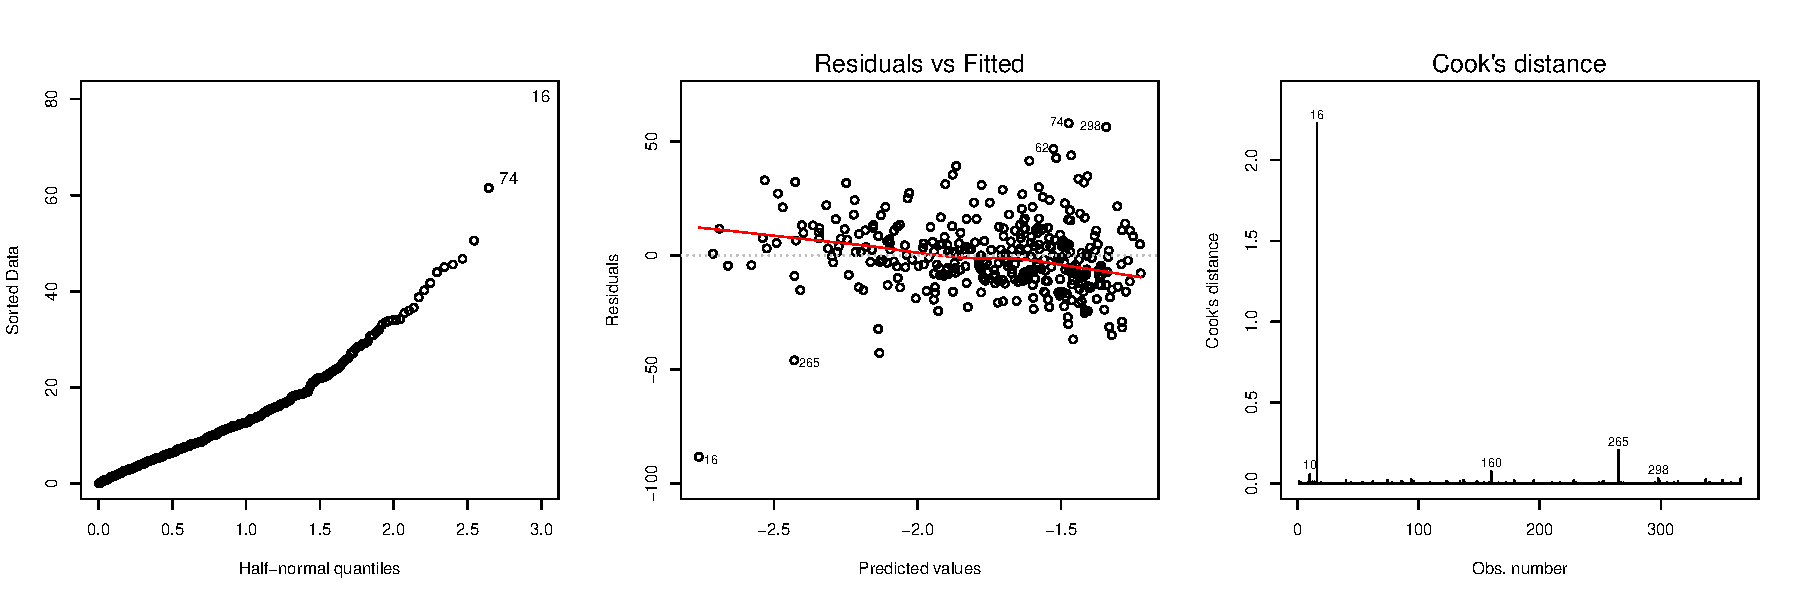
\includegraphics{Report_files/figure-latex/unnamed-chunk-15-1} 

}

\caption{\label{ass_mdl2}Diagnostics first quasi-binomial model}\label{fig:unnamed-chunk-15}
\end{figure}

The left plot of figure \ref{ass_mdl2} visualizes the half-normal
quantiles against the pearson residuals. Ideally, these residuals would
not be greater than 3. However, this plot shows residuals even up to 80.
The middle plot displays the predicted values against the deviance
resiuals. Also here a large spread of the residuals is observed and the
variance tends to increase with an increase of the fitted value. The
right plots visualizes the cook's distance, which can identify
influential observations. Observation 16 is an outlier, because it is
very influential and stands out from any pattern in the residual plots.
Furthermore, Dinkelland (obs 74) and Rotterdam (obs 265) are also
influential. Amsterdam is the municipality with the lowest percentage of
CDA votes and Dinkelland has the highest percentage of CDA votes.

\begin{figure}[H]

{\centering 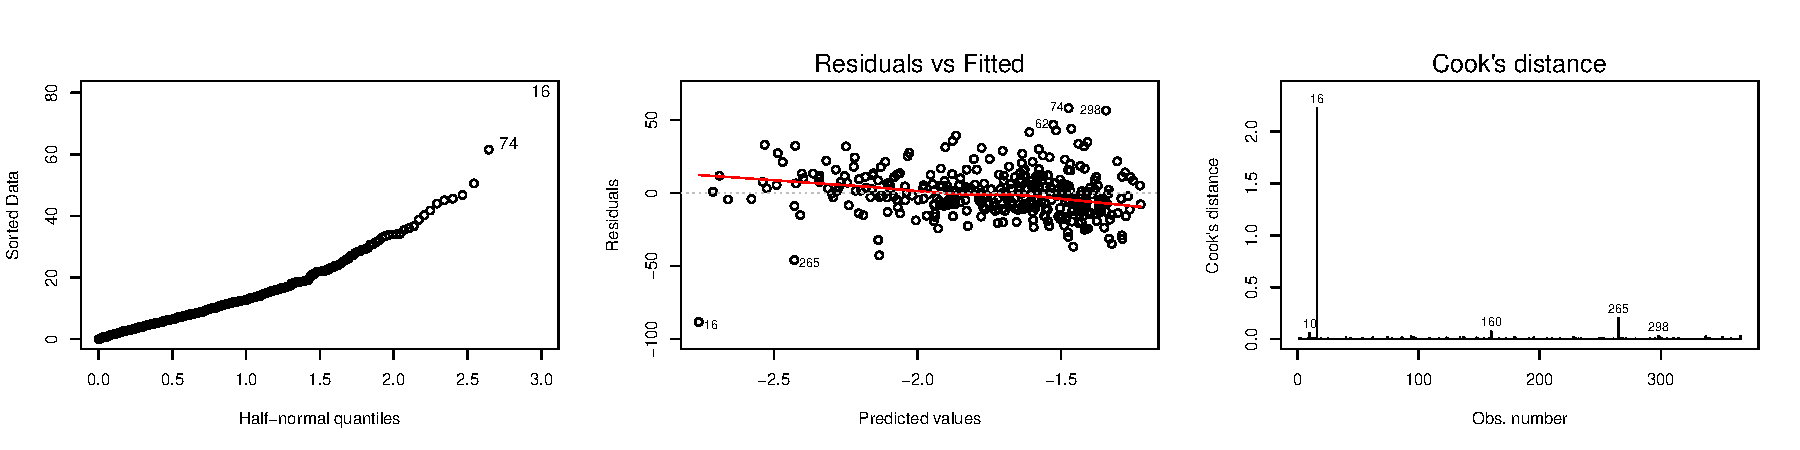
\includegraphics{Report_files/figure-latex/unnamed-chunk-16-1} 

}

\caption{\label{av_mdl2}AvPlots first quasi-binomial model}\label{fig:unnamed-chunk-16}
\end{figure}

Figure \ref{av_mdl2} help to interpret the partial regression
coefficients in a model when the other variables are held constant. The
partial regression line is highly influenced by observation 16 again.
The blue lines do not represent the data well at the moment.

\subsection{3.3 Third model}\label{third-model}

For this model the variable \texttt{Frac\_60plus} is removed, because it
had the lowest F-value. Furthermore, the observations 16 (Amsterdam) and
265 (Dinkelland) are removed. These influence the partial regression
coefficients greatly and have large residuals and cook's distances.
These steps were originally done in two, but are combined for this
report.

Below the summary output from this third model:

\begin{table}[ht]
\centering
\begin{tabular}{rrrrr}
  \hline
 & Estimate & Std. Error & t value & Pr($>$$|$t$|$) \\ 
  \hline
(Intercept) & -1.0878 & 0.1802 & -6.04 & 0.0000 \\ 
  Urban\_index & -0.1352 & 0.0303 & -4.46 & 0.0000 \\ 
  High\_educated\_frac & -1.2202 & 0.3126 & -3.90 & 0.0001 \\ 
  Mean\_income & -0.0004 & 0.0082 & -0.05 & 0.9583 \\ 
  Non\_west2 & -0.1232 & 0.0479 & -2.57 & 0.0105 \\ 
  Non\_west3 & -0.3447 & 0.0691 & -4.99 & 0.0000 \\ 
   \hline
\end{tabular}
\end{table}

By removing observation 16 and 265, the factor \texttt{Non\_west2} has
become significant. The null deviance has dropped to 173,842 with 363 df
and the residual deviance has decreased slightly to 76,966 with 358 df.
\(\phi\) has increased slightly to 221.709.

\begin{figure}[H]

{\centering 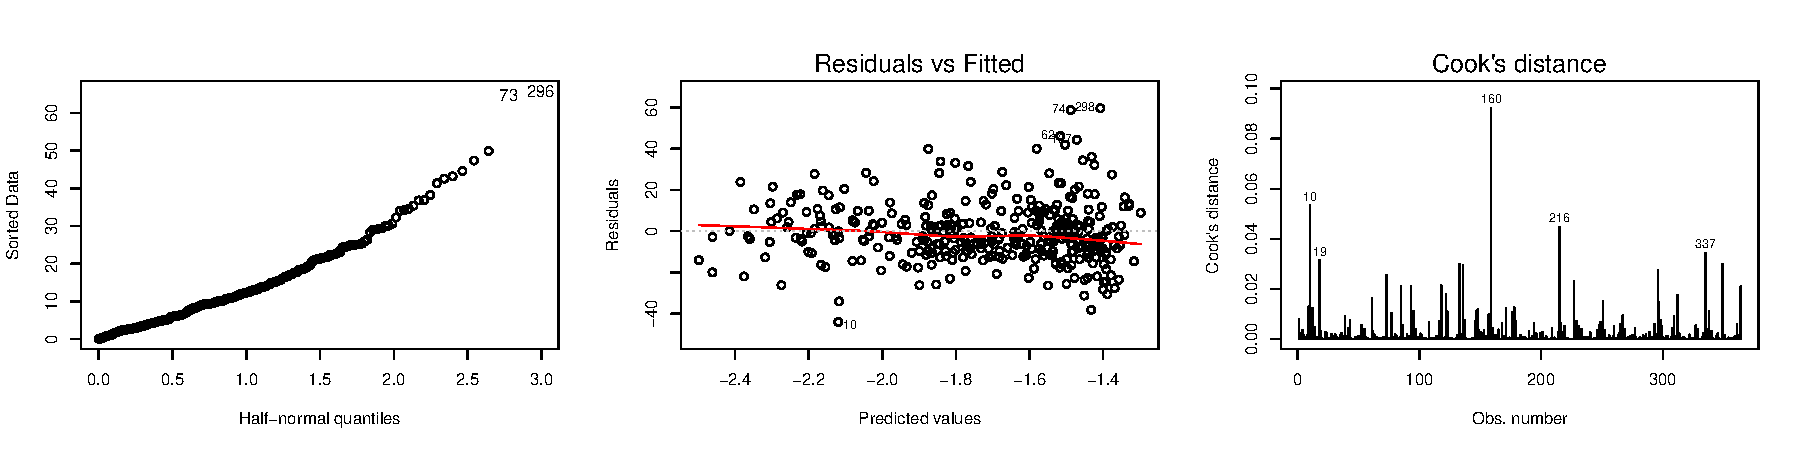
\includegraphics{Report_files/figure-latex/unnamed-chunk-18-1} 

}

\caption{\label{ass_mdl3}Diagnostics third quasi-binomial model}\label{fig:unnamed-chunk-18}
\end{figure}

The plot left still displays very large pearson residuals. The plot in
the middle still visualized that the deviance residuals tend to increase
when the predicted values increase. The cook's distance no longer
displays highly influential observations.

\begin{table}[ht]
\centering
\begin{tabular}{lrrrr}
  \hline
 & Df & Deviance & F value & Pr($>$F) \\ 
  \hline
$<$none$>$ &  & 76965.83 &  &  \\ 
  Urban\_index & 1 & 81395.63 & 20.60 & 0.0000 \\ 
  High\_educated\_frac & 1 & 80361.41 & 15.79 & 0.0001 \\ 
  Mean\_income & 1 & 76966.44 & 0.00 & 0.9577 \\ 
  Non\_west & 2 & 82994.45 & 14.02 & 0.0000 \\ 
   \hline
\end{tabular}
\end{table}

According to the F-test \texttt{Mean\_income} should be removed as well,
because the F-value is below 1 and the corresponding p-value is 0.96.

\subsection{3.4 Final model}\label{final-model-1}

The final model is reached after dropping the variable
\texttt{Mean\_income}. It's formula is as follows:

\(logit(\theta_{i}) = -1.09 -0.13 \cdot UrbanIndex -1.23 \cdot HighlyEducatedFraction - 0.12 \cdot NonWest2 - 0.34 \cdot NonWest3 + \epsilon_i\)

The summary output is as follows:

\begin{table}[ht]
\centering
\begin{tabular}{rrrrr}
  \hline
 & Estimate & Std. Error & t value & Pr($>$$|$t$|$) \\ 
  \hline
(Intercept) & -1.0965 & 0.0653 & -16.80 & 0.0000 \\ 
  Urban\_index & -0.1350 & 0.0300 & -4.50 & 0.0000 \\ 
  High\_educated\_frac & -1.2297 & 0.2541 & -4.84 & 0.0000 \\ 
  Non\_west2 & -0.1235 & 0.0477 & -2.59 & 0.0100 \\ 
  Non\_west3 & -0.3444 & 0.0688 & -5.01 & 0.0000 \\ 
   \hline
\end{tabular}
\end{table}

\begin{table}[ht]
\centering
\begin{tabular}{lrrrr}
  \hline
 & Df & Deviance & F value & Pr($>$F) \\ 
  \hline
$<$none$>$ &  & 76966.44 &  &  \\ 
  Urban\_index & 1 & 81470.68 & 21.01 & 0.0000 \\ 
  High\_educated\_frac & 1 & 82189.93 & 24.36 & 0.0000 \\ 
  Non\_west & 2 & 83076.91 & 14.25 & 0.0000 \\ 
   \hline
\end{tabular}
\end{table}

According to the F-test all variables now significantly contribute to
the model. The null deviance is still 173,842 with 363 df and the
residual deviance has slightly decreased to 76,966 with 359 df. \(\phi\)
is estimated at 221.1.

\begin{figure}[H]

{\centering 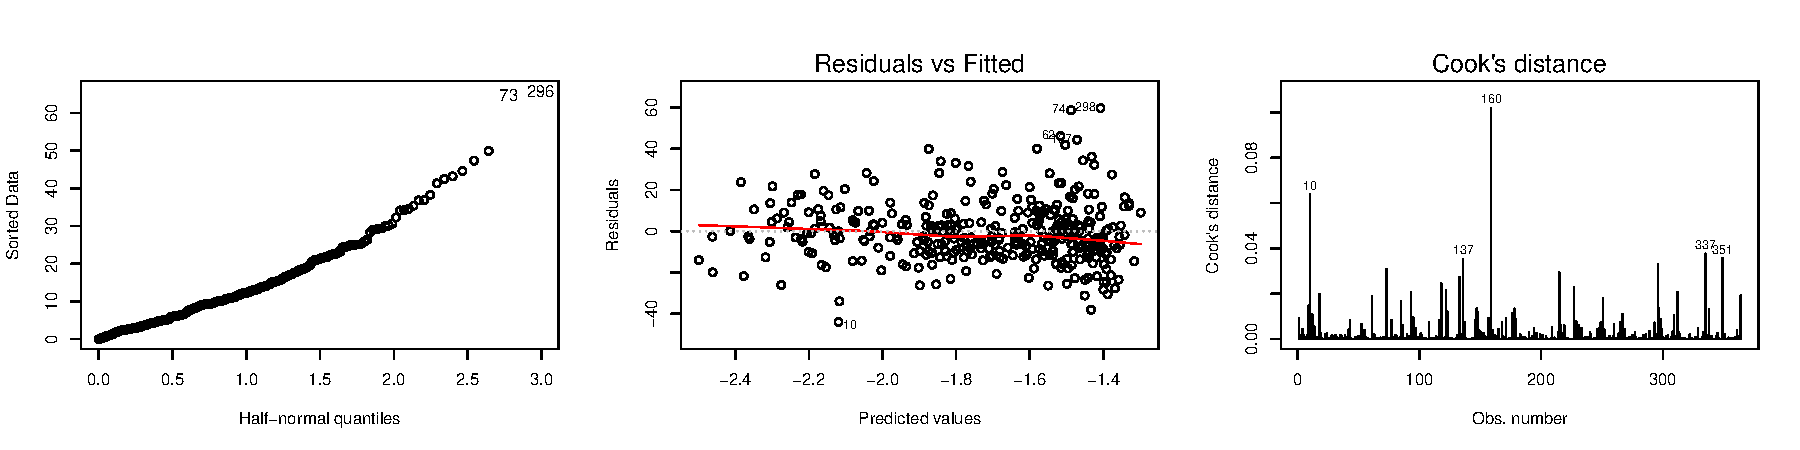
\includegraphics{Report_files/figure-latex/unnamed-chunk-21-1} 

}

\caption{\label{ass_final}Diagnostics final quasi-binomial model}\label{fig:unnamed-chunk-21}
\end{figure}

Figure \ref{ass_final} displays that there is still a large spread of
both the pearson (left plot) and deviance (middle plot) residuals.
Furthermore, there is non-constant errror variance. The cook's distance
does not display very influential observations.

\begin{figure}[H]

{\centering 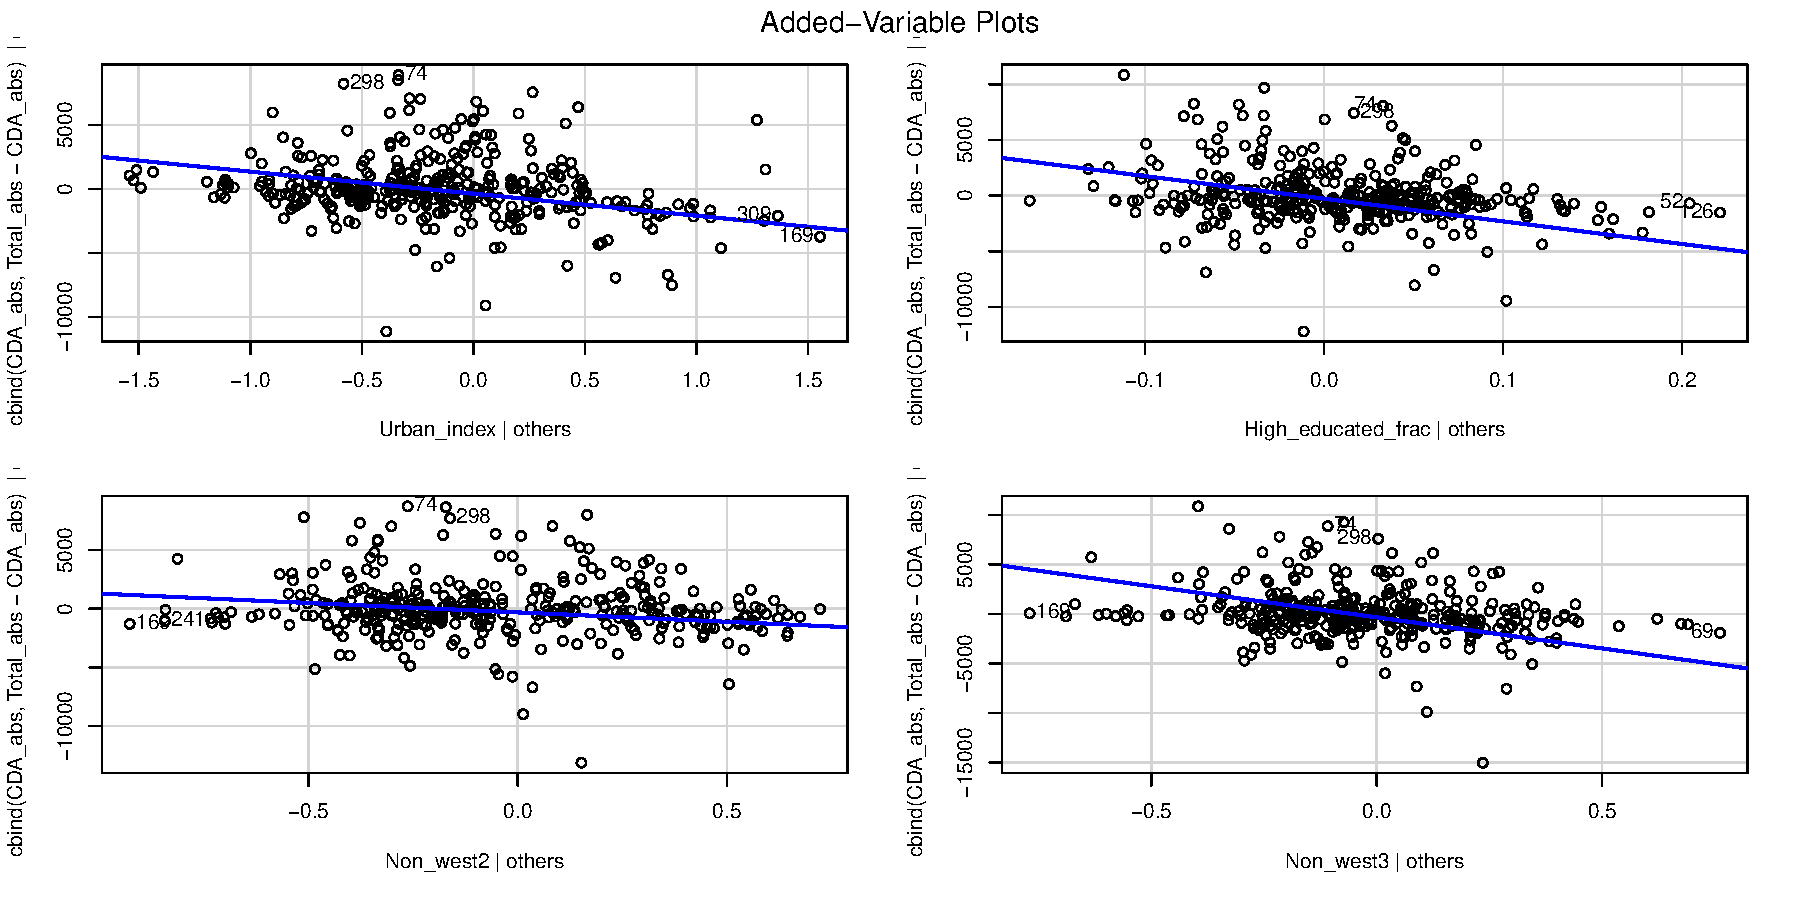
\includegraphics{Report_files/figure-latex/unnamed-chunk-22-1} 

}

\caption{\label{av_final}Diagnostics final quasi-binomial model}\label{fig:unnamed-chunk-22}
\end{figure}

\begin{verbatim}
##        Urban_index High_educated_frac          Non_west2 
##       0.0012896670       0.0004230904       0.0007928046 
##          Non_west3 
##       0.0012734699
\end{verbatim}

After removing two outliers, the partial regression coefficients
represent the data much better. There are no strong correlations between
the explanatory variables and the respons. The low VIF values also
indicate this.

\subsection{3.5 Cross validation}\label{cross-validation-1}

At last, the logistic model is validated by k-fold validation. This
dataset has 366 observations, therefore K = 5 is enough. The code for
cross validation is similar to the one used for the linear model.
Therefore, only the output is presented here and not the code.

\begin{verbatim}
## [1] 0.001707315
\end{verbatim}

The cross validation results in a Prediction Means Squared Error (PMSE)
of 0.0017.

\section{4. Discussion}\label{discussion}

\subsection{4.1 Multiple Linear
regression}\label{multiple-linear-regression-1}

Because the fitted values are transformed to a log form, it is also
possible to raise the coëfficients to a exponential power. The final
model obtained then is:

\(Y_i = e^{-1.0298 -0.8277 \cdot HighEducatedFraction -0.1311 \cdot Urban Index -0.1141 \cdot Non west2 -0.2871 \cdot Non west3 -3.0168 \cdot Frac 60plus + \epsilon_i}\)

Per variable the influence will be discussed. The slope will start at
point \(exp(-1.0298)\), this is equal to 0.357. This means if all the
other demographic variables are zero, the fitted value will be equal to
the intercept, so equal to 0.357. This not a possible outcome, because a
Municipality with all these demographics equal to zero is not a reality.

For the other coefficients it is a bit harder to predict there
influence, because of the log transformation and the different range the
variables have. For example, the \emph{Urban Index} has a 0-3.8 range
and \emph{Highly educated} has a 0.12-0.47 range in this data set. But
still some remarks can be made about the slope of the model. The
\emph{Fraction 60 plus} has the lowest marginal impact on the slope, if
all variables are hold constant and \emph{Frac 60 plus} changes with one
unit, then the exponent changes with -3.02. The \emph{Non west2} has the
highest impact on the slope, because the coefficient is the lowest.

The outcome of the cross validation for this model is 0.0582. Hence, the
predicted mean squared difference between the fitted and predicted value
is 0.0582, which is very close to 0.

There are some limitations for this model, because the response variable
is a fraction and will never be larger than one, theoratically a
logistic regression would fit the data better. Also some assumptions are
violated. In the fitted vs residual graph it is visible that the
variance is not equally spread, there is a small ``loudspeaker
pattern''. But because the fitted values are log transformed, it is not
really possible to adapt this any further. Also there are two
municipalities that fall outside the {[}-3,3{]} range in the normality
plot, but because they are still in the 95\% envelope the decision is
made to not delete these municipalities.

\subsection{4.2 Logistic regression}\label{logistic-regression-1}

For the final model two variables and two outliers are removed. The
coefficients of the model are on the log-odds scale and need to be
transformed before interpretating them. Each estimated coefficient is
the expected change in the log odds of voting for CDA for a unit
increase in the corresponding explanatory variable holding the other
explanatory variables constant.

The coefficient for \emph{Urban Index} is the difference in the log
odds. In other words, the expected change in log odds of voting for CDA
is -0.13. This can be transformed to the odds: \(exp(-0.13)\) = 0.88.
The odds of voting for CDA decrease with roughly 12\% if the Urbanity
increases with one unit. The Urbanity index has a range from 0 to 4, so
this variable has a large influence. For example, when comparing
Terschelling (Urbanity index of 0) and Leiden (Urbanity index of 3.7),
the expected decrease is 40.7\%.

An similar calculation can be done for one unit increase of \emph{Non
west}. When \emph{Non west} increases from 1 (the reference level) to 2
and the other explanatory variables are held constant, then the log odds
of voting for CDA is -0.12. Transforming this to the odds results in a
decrease of 11\%, roughly. And when when comparing factor level 1 to 3,
the log odds is -0.34. This results in the odds of \(exp(-0.34)\) =
0.71, a decrease of 29\%. This is not a simple duplication of level 2.

According to the model, holding \emph{Highly educated} and \emph{Non
west} constant, the odds of voting for CDA if the Urban index increases
with 1 unit is \(exp(-0.16)\) = 0.87. In percentage change does this
mean that the odds decrease with 12.6\%.

At last, the odds of voting for CDA if \emph{Highly educated} increases
with 1 unit is \(exp(-1.23)\) = 0.29. In percentage change does this
mean that the odds decrease with 70.8\%. This is a very large decrease,
but can be explained. This variable is a fraction and has a range from 0
- 1. An increase of one unit is not likely to happen.

In summary, municipalities in rural areas, with smaller amounts of
Non-western and Highly educated residents tend to vote for CDA. Below
the formula with the odds ratio is shown:

\((\frac{\theta_i}{1 - \theta_i}) = 0.33 + 0.88 \cdot UrbanIndex + 0.29 \cdot HighlyEducatedFraction - 0.89 \cdot NonWest2 + 0.71 \cdot NonWest3 + \epsilon_i\)

As already said, there is still dispersion, even after using a quasi
binomial model. A possible explanation can be clustering of
observations. Municipalities close to each other will probably vote
similar. Figure \ref{Results elections} shows that the municipalites
where CDA (shown in light green) is the biggest party are clustered
together. CDA is the biggest party in large parts of Friesland,
Groningen and Drente. The municipalities located here probably have a
similar population.

\begin{figure}
\centering
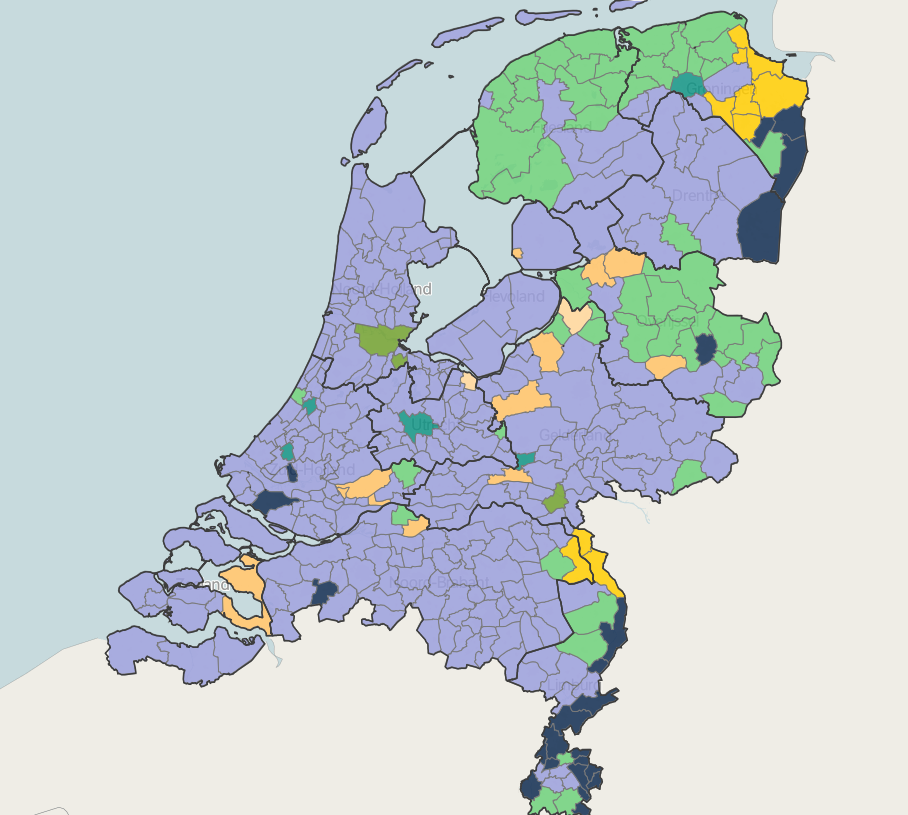
\includegraphics[width=2.60417in]{Uitslag_verkiezingen2017.png}
\caption{\label{Results elections}Results elections with biggest
parties. CDA is displayed in light green}
\end{figure}

Another explanation for the dispersion is the large variation. In some
municipalities only 3\% voted for CDA, while in other almost 50\%. This
large variation is hard to modeled in a binomial. By using the log odds,
votes are distributed in two groups: voted for CDA or not voted for CDA.
However, with 13 political parties is it hard to distinguish two groups.
Because it is not possible take to into account which parties are
similar to CDA.

Even though, the cross validation resulted in a PMSE of 0.0017, it is
not likely that this model can make future predictions. This because of
the large overdispersion and non-constant error variance.

\subsection{4.3 Further research}\label{further-research}

Both of the models have different significant variables. This makes it
even more difficult to determine which model is better fitting. However,
the logistic regression fits the underlying pattern of the data better
and has a smaller MSPE. Further research into the correctness of the
models should be done. Another topic that can be researched in further
research is the influence of demographics on districts of municipalities
instead of the whole municipialities. Right now the developed models
nullified the differences in demographics between areas in a
municipality.


\end{document}
